\documentclass{article}
\usepackage{graphicx} % Required for inserting images

\title{Polynomial Multiplication with Parallelized FFT writeup}
\author{Alex Pan}
\date{April 2024}

\usepackage[margin=1in]{geometry}
\usepackage{amsmath}
\usepackage{amsfonts}
\usepackage{hyperref}
\usepackage{parskip}
\usepackage{wasysym}
\usepackage{adjustbox}

\begin{document}

\maketitle

\textbf{Everything before section 7 (hypertriangle) isn't useful for raising multivariate polynomials to powers.}

This is because FFT in $k$-dimensions has a time complexity of $O(n^k \log{n})$. FFT in $1$ dimension is $O(n\log{n})$, and in $k$ dimensions, the $1$-D FFT needs to be repeated roughly $n^{k-1}$ times, making the total complexity $O(n^k \log{n})$. So, even with the number of applications FFT has, it isn't the best choice when raising higher-dimensional polynomials to powers.
\section{Overview}
Using the Fast Fourier Transform (FFT), we can multiply two univariate polynomials of in $O(n\log(n))$ time, compared to the trivial distributive algorithm of $O(n^2)$. In addition, this process is fully parallelizable, making its computation extremely quick using GPUs. In order to understand the algorithm, we need to understand a few steps:

\begin{itemize}
    \item Polynomial Interpolation 
    \item DFT and FFT
    \item Parallelization
\end{itemize}

\section{Polynomial Interpolation}
Given a set of $n+1$ points $(x_0,y_0), (x_1,y_1) ... (x_n, y_n)$, with all $x_i$ being distinct, there exists a unique polynomial of degree \textit{at most} $n$ that passes through all $n+1$ points.

To verify this, we start by writing the polynomial $p(x)$ as $a_0 + a_1x^1 + a_2x^2 + ... + a_nx^n$, we can write this as a matrix product:

\centerline{$\begin{bmatrix} 1 & x & x^2 & \ldots & x^n \end{bmatrix}\begin{bmatrix} a_0 \\ a_1 \\ a_2 \\ \vdots \\ a_n \end{bmatrix} = p(x) = y$}

Doing this for all $x_i$, we get the \textit{Vandermonde Matrix} and the equation:

\centerline{
    $
    \overbrace{
        \begin{bmatrix}
            1 & x_0 & x_0^2 & \ldots & x_0^n \\
            1 & x_1 & x_1^2 & \ldots & x_1^n \\
            1 & x_2 & x_2^2 & \ldots & x_2^n \\
            \vdots & \vdots & \vdots & \ddots & \vdots \\
            1 & x_n & x_n^2 & \ldots & x_n^n \\
        \end{bmatrix}
    }^{\text{\large $V$}}
    \overbrace{
        \begin{bmatrix}
            a_0 \\ a_1 \\ a_2 \\ \vdots \\ a_n 
        \end{bmatrix}
    }^{\text{\large $\vec{a}$}} = 
    \begin{bmatrix}
        p(x_0) \\ p(x_1) \\ p(x_2) \\ \vdots \\ p(x_n) 
    \end{bmatrix} = 
    \overbrace{
        \begin{bmatrix}
            y_0 \\ y_1 \\ y_2 \\ \vdots \\ y_n 
        \end{bmatrix}
    }^{\text{\large $\vec{y}$}}
    $
}

To show that $\vec{a}$ is exists and is unique, we need to show that the Vandermonde matrix is bijective. Because it is square, we just need to verify that the matrix is invertible. From \href{https://en.wikipedia.org/wiki/Vandermonde_matrix}{Wikipedia}, the determinant of this matrix is nonzero if and only if all $x_i$ are distinct, which we specified earlier. So, the polynomial represented by $\vec{a}$ exists and is unique, with $\vec{a}=V^{-1}\vec{y}$. (The non-linear algebra proofs are a lot more interesting)

An important comment to make is that the degree of the interpolated polynomial doesn't have to be $n$; the degree d can be any value from $1\le d\le n$ this is the case when $a_{d+1} \ldots a_n=0$. This means that given a set of data points, the interpolated polynomial will be of the lowest degree possible.

If we evaluate two polynomials $p(x)$ and $q(x)$ at a point $x_0$, then multiply their outputs together, we get the same value as if we multiplied the two polynomials first, then evaluated them at $x_0$. This forms the motivation for using polynomial interpolation to multiply polynomials.

The algorithm for multiplying polynomials $p(x)$ and $q(x)$, with coefficients $\vec{a}$ and $\vec{b}$ using interpolation is as follows:

\begin{enumerate}
    \item Determine degree $k$ of product: This is just the degrees of $p_1(x)$ and $p_2(x)$ added together: $n+m=k$
    \item Select arbitrary $k+1$ distinct values $x_0, x_1, \ldots, x_k$. Evaluate the polynomials at all of the values using the $(k+1)\times (k+1)$ Vandermonde matrix: $V\vec{a}=\vec{y}$, $V\vec{b}=\vec{z}$
    \item Perform component-wise multiplication on $\vec{y}$ and $\vec{z}$:

    \centerline{
        $
        \begin{bmatrix}
            y_0 \\ y_1 \\ y_2 \\ \vdots \\ y_k 
        \end{bmatrix} \circ
        \begin{bmatrix}
            z_0 \\ z_1 \\ z_2 \\ \vdots \\ z_k 
        \end{bmatrix} = 
        \begin{bmatrix}
            y_0z_0 \\ y_1z_1 \\ y_2z_2 \\ \vdots \\ y_kz_k 
        \end{bmatrix}
        $
    }
    \item Interpolate $\vec{y}\circ\vec{z}$ - find the unique polynomial that passes through all of the chosen points - compute $V^{-1}(\vec{y}\circ\vec{z})$
\end{enumerate}
This algorithm works, but runs in $O(n^3)$ time because finding the inverse of a matrix is $O(n^3)$, making it significantly slower than trivial multiplication. DFT fixes the finding the inverse part.

\section{DFT and FFT}
\subsection{DFT}
The Discrete Fourier Transform is a function maps a vector containing elements $[a_0, a_1, ... a_n]$ with $a_i\in \mathbb{C}$ to a vector containing elements $[\hat{a}_0, \hat{a}_1, ... \hat{a}_n]$ with the following rule:

$\hat{a}_k = \displaystyle\sum\limits_{j=0}^{n-1} x_j\cdot e^{-2\pi i \frac{k}{N}j}$

In the context of polynomial multiplication, DFT just evaluates a polynomial of degree $n$ at the $n$ complex roots of unity. So, with $\omega = e^{\frac{2\pi i}{n}}$ the Vandermonde matrix looks like this:

\centerline{
    $
    \overbrace{
        \begin{bmatrix}
            1 & 1 & 1 & \ldots & 1 \\
            1 & \omega & \omega^2 & \ldots & \omega^{n-1} \\
            1 & \omega^2 & \omega^4 & \ldots & \omega^{2(n-1)} \\
            \vdots & \vdots & \vdots & \ddots & \vdots \\
            1 & \omega^{n-1} & \omega^{2(n-1)} & \ldots & \omega^{(n-1)(n-1)} \\
        \end{bmatrix}
    }^{\text{\large $V$}}
    \overbrace{
        \begin{bmatrix}
            a_0 \\ a_1 \\ a_2 \\ \vdots \\ a_n 
        \end{bmatrix}
    }^{\text{\large $\vec{a}$}} = 
    \overbrace{
        \begin{bmatrix}
            y_0 \\ y_1 \\ y_2 \\ \vdots \\ y_n 
        \end{bmatrix}
    }^{\text{\large $\vec{y}$}}
    $
}

DFT is doing the same thing as the first step in the above algorithm, except it specifies the arbitrary points to be the $k$ roots of unity.

This is only useful because the inverse Vandermonde matrix $V^{-1}$ is already known - we don't need to calculate it:

\centerline{
    $ V^{-1} = \displaystyle\frac{1}{n}
    \begin{bmatrix}
        1 & 1 & 1 & \ldots & 1 \\
        1 & \omega^{-1} & \omega^{-2} & \ldots & \omega^{-(n-1)} \\
        1 & \omega^{-2} & \omega^{-4} & \ldots & \omega^{-2(n-1)} \\
        \vdots & \vdots & \vdots & \ddots & \vdots \\
        1 & \omega^{-1(n-1)} & \omega^{-2(n-1)} & \ldots & \omega^{-(n-1)(n-1)} \\
    \end{bmatrix}
    $
}

To verify: Checking entries on the diagonal, multiplying $\omega$ by its inverse $\omega^{-1}$ gives 1, and adding these up $n$ times and dividing by $n$ gives 1's on the diagonal. Checking entries not on the diagonal and in the first row or column, we see that adding the roots of unity just gives 0. I don't feel like proving the other entries.

With this, we no longer have to compute the inverse of the Vandermonde matrix in $O(n^3)$ time, and our algorithm has been shortened to $O(n^2)$, the complexity of multiplying a matrix by a vector. However, since we're doing so many extra steps, this algorithm is still slower, and requires more memory than the trivial algorithm.

\subsection{FFT}
Fast Fourier Transform in the context of Discrete Fourier Transforms refers to a fast way to compute $V\vec{a}=\vec{y}$. Given a polynomial $p(x)=a_0 + a_1x^1 + a_2x^2 + ... + a_{n-1}x^{n-1}$, and assuming that $n$ is a power of two, we can rewrite it as:

\begin{center}
    $p(x) = p_1(x^2) + x * p_2(x^2)$, where

    $p_1(x) = a_0 + a_2x + a_4x^2 + \ldots + a_{n-2}x^{\frac{n}{2}-1}$

    $p_2(x) = a_1 + a_3x + a_5x^2 + \ldots + a_{n-1}x^{\frac{n}{2}-1}$
\end{center}

This decomposition perfect for evaluating a polynomial at a complex root of unity. To see this, we look at the evaluation of a polynomial at the $n=8$ roots of unity using the decomposition above (this looks horrible but I'll live with it for a bit):
\begin{center}
    $
    \begin{bmatrix}
        p(
\includegraphics[height=1em]{icons/0.pdf}) \\ 
        p(\rotatebox[origin=c]{45}{
\includegraphics[height=1em]{icons/0.pdf}}) \\
        p(\rotatebox[origin=c]{90}{
\includegraphics[height=1em]{icons/0.pdf}}) \\
        p(\rotatebox[origin=c]{135}{
\includegraphics[height=1em]{icons/0.pdf}}) \\
        p(\rotatebox[origin=c]{180}{
\includegraphics[height=1em]{icons/0.pdf}}) \\
        p(\rotatebox[origin=c]{225}{
\includegraphics[height=1em]{icons/0.pdf}}) \\
        p(\rotatebox[origin=c]{270}{
\includegraphics[height=1em]{icons/0.pdf}}) \\
        p(\rotatebox[origin=c]{315}{
\includegraphics[height=1em]{icons/0.pdf}}) \\
    \end{bmatrix} =
    \begin{bmatrix}
        p_1(
\includegraphics[height=1em]{icons/0.pdf}) \\ 
        p_1(\rotatebox[origin=c]{90}{
\includegraphics[height=1em]{icons/0.pdf}}) \\
        p_1(\rotatebox[origin=c]{180}{
\includegraphics[height=1em]{icons/0.pdf}}) \\
        p_1(\rotatebox[origin=c]{270}{
\includegraphics[height=1em]{icons/0.pdf}}) \\
        p_1(
\includegraphics[height=1em]{icons/0.pdf}) \\ 
        p_1(\rotatebox[origin=c]{90}{
\includegraphics[height=1em]{icons/0.pdf}}) \\
        p_1(\rotatebox[origin=c]{180}{
\includegraphics[height=1em]{icons/0.pdf}}) \\
        p_1(\rotatebox[origin=c]{270}{
\includegraphics[height=1em]{icons/0.pdf}}) \\
    \end{bmatrix} + 
    \begin{bmatrix}
        
\includegraphics[height=1em]{icons/0.pdf}p_2(
\includegraphics[height=1em]{icons/0.pdf}) \\ 
        \rotatebox[origin=c]{45}{
\includegraphics[height=1em]{icons/0.pdf}}p_2(\rotatebox[origin=c]{90}{
\includegraphics[height=1em]{icons/0.pdf}}) \\
        \rotatebox[origin=c]{90}{
\includegraphics[height=1em]{icons/0.pdf}}p_2(\rotatebox[origin=c]{180}{
\includegraphics[height=1em]{icons/0.pdf}}) \\
        \rotatebox[origin=c]{135}{
\includegraphics[height=1em]{icons/0.pdf}}p_2(\rotatebox[origin=c]{270}{
\includegraphics[height=1em]{icons/0.pdf}}) \\
        \rotatebox[origin=c]{180}{
\includegraphics[height=1em]{icons/0.pdf}}p_2(
\includegraphics[height=1em]{icons/0.pdf}) \\ 
        \rotatebox[origin=c]{225}{
\includegraphics[height=1em]{icons/0.pdf}}p_2(\rotatebox[origin=c]{90}{
\includegraphics[height=1em]{icons/0.pdf}}) \\
        \rotatebox[origin=c]{270}{
\includegraphics[height=1em]{icons/0.pdf}}p_2(\rotatebox[origin=c]{180}{
\includegraphics[height=1em]{icons/0.pdf}}) \\
        \rotatebox[origin=c]{315}{
\includegraphics[height=1em]{icons/0.pdf}}p_2(\rotatebox[origin=c]{270}{
\includegraphics[height=1em]{icons/0.pdf}}) \\
    \end{bmatrix}
    $ 
\end{center}

Note that with one recursive step, we only have to evaluate $p_1$ $p_2$, both with $n/2=4$ terms, at $n/2=4$ roots of unity. This is because when we square the roots of unity $\omega^{0}, \omega^{1}, \omega^{2},...,\omega^{n}$, we get $\omega^{0}, \omega^{2}, \omega^{4},...,\omega^{2n}$, the roots of unity generated by $\omega^{2}$, of which there are $n/2$ of. So, with each recursive decomposition, problem becomes evaluating two polynomials with half the size of the original polynomial at half of the roots of unity. Furthermore, letting $\omega_n$ be the $n$th root of unity, we see that $\omega_n^{n/2}=-\omega_n$, meaning we really only need to evaluate half of the second vector, and just need to negate the other half.

Note that letting $n$ be a different power $n=m^k$ gives access to a radix-m version of the recursive algorithm.

However, since we want to parallelize this, and not all NVIDIA GPUs support recursion yet, we need a way to build this algorithm bottom-up.

write cooley-tukey

Now our algorithm is $O(n \log_2n)$, asymptotically much better than our trivial $O(n^2)$ algorithm.

\section{Multinomial Multiplication}

The multidimensional version of this algorithm follows much of the same steps as the 1-dimensional algorithm. Given a polynomial of $k$ variables, we can represent its coefficients in a $k$-dimensional matrix/tensor $X$, We "DFT" $X$, multiply the corresponding coefficients of $X_1$ and $X_2$, and "IDFT" the result.

We need to define what the DFT in $k$ dimensions is first. A diagram from \href{https://link.springer.com/chapter/10.1007/978-1-4020-6629-0_5}{\textit{Fast Fourier Transform - Algorithms and Applications}} explains how the DFT works in 2 dimensions:

\begin{align*}
    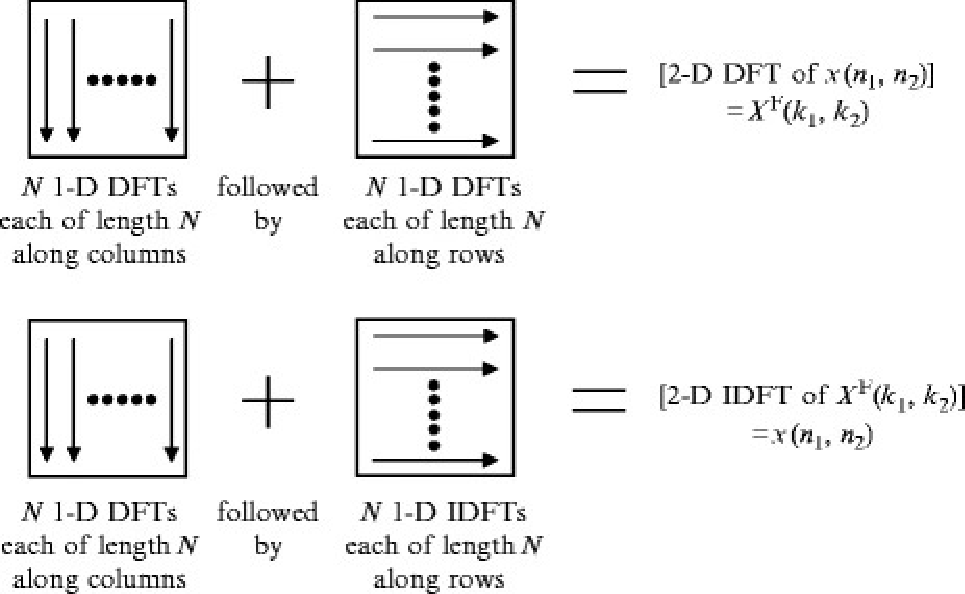
\includegraphics[height=20em]{icons/2ddft.pdf}
\end{align*}

So, in order to send a matrix/tensor to its frequency domain representation, we iteratively DFT each vector that makes up the matrix/tensor.

If the matrix is $n \times n$, then we need to apply $2n$ DFTs, each of complexity $O(n \log n)$, which already leads to a complexity of $O(n^2 \log n)$, already more than the trivial algorithm. The complexity of DFTing a $n \times n \times n$ tensor becomes $O(n^3 \log n)$, and generally, DFTing a $k$-dimensional tensor, each dimension with size $n$, will have complexity $O(n^k log n)$. 

Because the polynomials we are interested in multiplying are homogeneous, there is a small optimization we can make. The tensor representation of these polynomials will only have entries on their "opposite diagonal," or in the case of $dim > 2$, the entries will be on their "opposite diagonal slice" (I have no idea what vocabulary I should be using here). In the case of 2d, multiplying a matrix by an "opposite diagonal" matrix simply rotates the matrix and scales the entries, and in the case of $dim>2$, multiplying the tensor by an "opposite diagonal slice" tensor simply permutes the dimensions, depending on which dimension we're applying DFT to first, and scales the entries by values in the "opposite diagonal slice". This computation is $O(n^k)$, but extremely highly parallelizable, and I think it can just be embedded into a future DFT computation. This reduces the dimensions we have to DFT by one dimension, making our complexity $O(n^{k-1} log n)$.

\section{Parallelization}

\section{NTT}
(This stuff I don't fully understand, so I'm mostly just writing this for my own understanding)

Because the end goal is to multiply very high degree polynomials in $\mathbb{F}_p[x]$, (polynomials with coefficients that are elements $\mathbb{F}_p$, the field of integers mod $p$), the complex DFT starts to lose viability because of very large floats that lose precision, and there is no trivial way to embed mod p into $\mathbb{C}$

This is where the DFT over a ring comes in, which generalizes the complex root of unity method to all rings. The Vandermonde matrix is the same, except we need to replace $\omega_n=e^{\frac{2\pi i}{n}}$ with $\alpha$, where $\alpha$ is a principal $n$th root of unity ($n$ is the length of the vector we are transforming). In the case of fields, which $\mathbb{F}_p$ is, the principal $n$th root of unity just needs to satisfy $\alpha^k\ne1$ for $1\le k<n$, where the exponentiation is repeated multiplication. For the inverse DFT, if $n$ doesn't have a multiplicative inverse in $F$, then the transformation is not invertible. Also, if a principal $n$th root of unity doesn't exist, then the transformation won't work either.

To do a quick example, let's say we want to multiply $1+2x$ and $3+4x\mod 5$. Our expected result is $3+3x^2$, corresponding to a vector of $[3,0,3,0]$. Luckily, $2$ is a $n$th principal root of unity in $\mathbb{F}$: $2^1=2, 2^2=4, 2^3=3$. So:
\begin{align*}
    \begin{bmatrix}
        1 & 1 & 1 & 1 \\
        1 & 2 & 4 & 3 \\
        1 & 4 & 1 & 4 \\
        1 & 3 & 4 & 2 \\
    \end{bmatrix}
    \begin{bmatrix}
        1 \\
        2 \\
        0 \\
        0 \\
    \end{bmatrix}=
    \begin{bmatrix}
        3 \\
        0 \\
        4 \\
        2 \\
    \end{bmatrix}
    ,
    \begin{bmatrix}
        1 & 1 & 1 & 1 \\
        1 & 2 & 4 & 3 \\
        1 & 4 & 1 & 4 \\
        1 & 3 & 4 & 2 \\
    \end{bmatrix}
    \begin{bmatrix}
        3 \\
        4 \\
        0 \\
        0 \\
    \end{bmatrix}=
    \begin{bmatrix}
        2 \\
        1 \\
        4 \\
        0 \\
    \end{bmatrix}
\end{align*}
\begin{align*}
    \begin{bmatrix}
        3 \\
        0 \\
        4 \\
        2 \\
    \end{bmatrix}\circ
    \begin{bmatrix}
        2 \\
        1 \\
        4 \\
        0 \\
    \end{bmatrix}=
    \begin{bmatrix}
        1 \\
        0 \\
        1 \\
        0 \\
    \end{bmatrix}
\end{align*}
\begin{align*}
    4
    \begin{bmatrix}
        1 & 1 & 1 & 1 \\
        1 & 3 & 4 & 2 \\
        1 & 4 & 1 & 4 \\
        1 & 2 & 4 & 3 \\
    \end{bmatrix}
    \begin{bmatrix}
        1 \\
        0 \\
        1 \\
        0 \\
    \end{bmatrix}=
    \begin{bmatrix}
        3 \\
        0 \\
        3 \\
        0 \\
    \end{bmatrix}
\end{align*}

So, we do indeed get the right output as our vector.
However, we won't necessarily be so lucky to have an $n$th principal root of unity, and we absolutely won't have a principal root of unity when the degree of the polynomial is greater than the order of the field. So, we instead need to look at $GF(p^n)$


\section{Pascal's Hypertriangle (Pascal's Simplex)}
Just as Pascal's Triangle is referenced to compute the coefficients of each term in a binomial expansion, Pascal's simplex can be used to compute the coefficients of each term in a multinomial expansion.

Say we want to compute $(a_0 + a_1 + ... + a_k)^n$. The coefficient in front of the term $a_0^{d_0}a_1^{d_1}...a_k^{d_k}$ can be computed by $\frac{n!}{d_0!d_1!...d_k!}$. For example, if we wanted to expand $(a + b + c)^3$, then the coefficient in front of $a^2 b$ would be $\frac{3!}{2!1!0!}=2$. Note that the sum of all of the degrees of the result equals $n$, or $\sum_{i=0}^{k} d_i=n$

Using stars and bars (distributing $n$ degrees amongst $k$ variables), we find that we have to compute $n + k - 1 \choose k-1$ coefficients.

The intuitive way to apply this is to compute all of the coefficients, and given a multinomial, map every $n + k - 1 \choose k-1$ term to the coefficient in front of it, and add all of them up.

\textbf{Easy Multinomial Expansion Algorithm (our current one)}

Given a multinomial and a power: $(a_1 + a_2 + ... + a_k)^n$, where $a_i$ represents a term $c_ix^py^qz^r...$

\begin{enumerate}
    \item Generate all $\binom{n+k-1}{k-1}$ possible terms of the expansion, store into array termPowers. termPowers will be a 2d array , with elements looking like $(d_1, d_2, ... , d_k)$. Initialize result array with same length as termPowers.
    \item Encode all monomials of the multinomial. Use the base-number conversion method: if the resulting degree is 20, and the monomial is of form $c_ix^py^qz^r...$, then the encoded form is a tuple $(c_i, 20^0 * p + 20^1 * q + 20^2 * r)$. Note that this encoding is homomorphic: $(x^2yz)^5$ has resulting degree $20$, so encode it as $800 + 20 + 1 = 821$. $821*5 = 4105 = 10 * 400 + 5 * 20 + 5 \rightarrow x^{10}y^5z^5$
    \item Iterate through every index of termPowers. Compute the multinomial coefficient, which will be $\frac{n!}{d_1!d_2!...d_k!}$. Raise $c^d_i$ for each index $i$ in $(d_1, d_2, ... , d_k)$, and multiply $c$ by the multinomial coefficient. Also compute the resulting degrees of the variables, and send to result.
    \item Sort result by the encoded monomials.
    \item reduce the result by key, where the keys are the encoded monomials ?????????
    \item decode all monomials
    \item return result
\end{enumerate}






\textit{Theorem}: Let $g$ be a multinomial of $k$ terms, where $k \ge p$, and degree $k$. If $maxCoef(g) \le M$, then $maxCoef(g^p) \le p! M^p,$ where \textbf{$g^p$ is unreduced}

\textit{Proof}: The multinomial coefficient of each resulting term is computed by $\frac{p!}{d_{1}!...d_{p}!}$. With the initial condition that the number of terms is greater than $p$, this tells us that the maximum multinomial coefficient is $\frac{p!}{1!...1!} = p!$. The maximum coefficient is $M^p$, which happens when there are at least $p$ starting terms of coefficient $M$. Multiplying these together, we get that the maximum coefficient of $g^p$ is bounded above by $p! M^p$

The theorem above is kind of useless. It doesn't consider what happens when like terms are combined.

\textit{Conjecture}: Let $g$ be a polynomial of $k$ variables and homogeneous $k$ degree. Let $maxCoef(g) < M$. Then, $maxCoef(g^p)$ is bounded by $M^p$ times the corresponding entry in \href{https://oeis.org/A333901/internal}{OEIS A333901} (genuinely wtf? where do primes even come in here?), where $n$ is $p$ and $k$ is $k$. The matrix is symmetric.

\textit{reason for conjecture}: Bunch of empirical data generated with multivariate algorithms/testing.jl

conclusion: chinese remainder theorem looks very necessary, those numbers get big fast

\textit{Conjecture}: If $g$'s terms are all possible monomials of $k$ variables and degree $k$, then $g^p$'s terms will be all possible monomials of $k$ variables and degree $pk$.

\textit{reason for conjecture}: I don't actually know if it's true, but all monomials I thought of could be represented

Benchmarking some cases of interest:
Let $g$ be a polynomial of $k$ variables and homogeneous $k$ degree that we want to raise to the $p$.

The maximum \# of starting terms is given by $\binom{2k-1}{k}$. This comes from stars and bars with $k$ stars and $k$ bars.

The maximum \# of ending, unreduced terms is given by $\binom{p + \binom{2k-1}{k} - 1}{p}$

The maximum \# of ending, reduced terms is given by $\binom{pk + k - 1}{k - 1}$

What we are really interested in is what happens when we raise a polynomial to the $p-1$ mod p and then to the $p$.

If we start with $k = 4$ and $p = 5$, then the maximum coefficient of $g^{p-1}$ is $p - 1 = 4$ because we're working in $\mathbb{F}_p$. $g^p$ has a maximum of $969$ reduced terms $(\binom{16+4-1}{3})$. All of the monomials are of degree $16$

Then, raising a polynomial of $969$ terms to the $5$ results in $37115800155$ resulting unreduced terms, which is out of the scope of our cpu algorithm for generating compositions. Reducing, we get $91881$ terms.

The OEIS thing isn't enough, need another formula that takes numVars, degree, and power to compute the maximum coefficient.



\end{document}

